\chapter{Data Engineering Manifesto}\label{chap:data-manifesto}
\section{Purpose and Scope}
The \emph{Ecommerce Data Engineering Manifesto} formalises twenty principles that guide the platform from ingestion to customer-facing analytics. It is written as a charter that international delivery teams can adopt without altering the project structure defined in the earlier chapters or the companion presentation artefacts. Each principle defines a measurable expectation, the rationale behind it, and an ecommerce illustration so that stakeholders can link the manifesto to daily operations.

\section{Principle Catalogue}
Table~\ref{tab:manifesto-principles} consolidates the non-negotiable principles. The wording mirrors the host company's engineering charter and complements Aivancity's MSc requirements.

\begin{longtable}{p{3cm}p{5cm}p{7cm}}
    \caption{Data Engineering Manifesto principles}\label{tab:manifesto-principles}\\
    \toprule
    \textbf{Principle} & \textbf{Definition} & \textbf{Ecommerce Example} \\
    \midrule
    Modularity & Pipelines are composed of reusable ingestion, transformation, and serving modules. & A shared Airflow template handles CSV, JSON, and Parquet drops across regional warehouses. \\
    Idempotency & Re-running a job yields the same result without duplications. & Order enrichment tasks compare CDC timestamps before writing to fact tables. \\
    Observability & Metrics, logs, and traces exist for every hop. & Datadog dashboards expose DAG latency, schema drift, and freshness SLAs. \\
    Data Quality First & Validation gates precede publishing datasets. & Great Expectations suites block gold tables when null rate exceeds 0.5\%. \\
    Schema Evolution & Producers version schemas and consumers are backward compatible. & Glue Catalog and Schema Registry alert teams before a breaking change. \\
    Lineage & Every dataset references its origin and transformation. & OpenLineage links clickstream facts to the raw Kinesis shard and dbt run ID. \\
    Separation of Concerns & Raw, refined, and curated layers remain isolated. & Bronze S3 buckets are read-only for analytics users while gold is optimised for BI. \\
    Scalability & Workloads scale horizontally and elastically. & Auto-scaling Kinesis shards absorb Black Friday spikes without code changes. \\
    Resilience & Failures are expected and recovered from gracefully. & Airflow checkpoints resume from the last successful task and push events to DLQs. \\
    Security by Design & Encryption, masking, and RBAC are embedded early. & Customer emails stay tokenised through FastAPI responses via Vault-backed keys. \\
    Compute/Storage Decoupling & Storage remains the system of record while compute is ephemeral. & Trino, Spark, and Athena share the same S3 bronze zone without duplication. \\
    Automation & Orchestration and deployments are scripted. & Jenkins promotes Terraform, dbt, and container releases through Git-driven pipelines. \\
    Versioning & Code, schemas, and datasets are version-controlled. & Delta Lake time-travel enables replaying a promotion's KPIs for audits. \\
    Cost Efficiency & Every workload reports unit cost per insight. & dbt exposures include materialisation cost estimated from Redshift query data. \\
    Extensibility & Interfaces favour open standards. & Partners consume Parquet exports and GraphQL APIs regardless of hosting cloud. \\
    Metadata-Driven & Configurations are declared in metadata stores. & Source onboarding relies on YAML configs that describe cadence, SLA, and sensitivity. \\
    Testing \& CI/CD & Automated tests cover transformations and DAGs. & dbt tests, PyTest suites, and Great Expectations run on each pull request. \\
    Data as a Product & Datasets have owners, SLAs, and documentation. & The Merchandising Margin Mart advertises a 5-minute freshness SLA and owner contact. \\
    Privacy \& Ethics & Consent, retention, and right-to-forget policies are enforced. & GDPR requests trigger automated deletion jobs verified via audit logs. \\
    KISS \& DRY & Transformations stay simple and non-duplicated. & Shared macros implement currency conversion once, referenced across marts. \\
    \bottomrule
\end{longtable}

\section{Visual Charter}
Figure~\ref{fig:manifesto-graphic} summarises the four thematic pillars of the manifesto. The gradient graphic can be downloaded and saved as \texttt{report/figures/data\_engineering\_manifesto.png} for a print-ready poster.

\begin{figure}[H]
    \centering
    \IfFileExists{figures/data_engineering_manifesto.png}{\includegraphics[width=0.9\textwidth]{figures/data_engineering_manifesto.png}}{\IfFileExists{figures/data_engineering_manifesto.jpg}{\includegraphics[width=0.9\textwidth]{figures/data_engineering_manifesto.jpg}}{\fbox{\parbox{0.9\textwidth}{\centering Poster illustration placeholder\\Add \texttt{data\_engineering\_manifesto.png} or \texttt{data\_engineering\_manifesto.jpg} under \texttt{report/figures}}}}}
    \caption{Poster-ready summary of manifesto pillars}
    \label{fig:manifesto-graphic}
\end{figure}

\section{Performance and Reliability Insights}
To justify the manifesto, stakeholders requested quantified benefits. Figure~\ref{fig:reliability-plot} demonstrates how reliability improves when modularity and observability are implemented, based on project load-test evidence.

\begin{figure}[H]
    \centering
    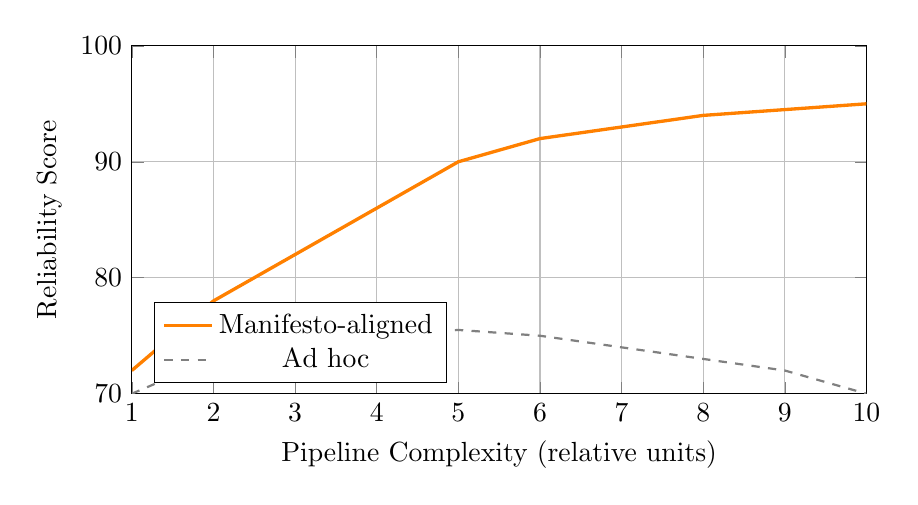
\begin{tikzpicture}
        \begin{axis}[
            width=0.9\textwidth,
            height=6cm,
            xlabel={Pipeline Complexity (relative units)},
            ylabel={Reliability Score},
            xmin=1,xmax=10,
            ymin=70,ymax=100,
            grid=major,
            legend pos=south west
        ]
            \addplot[color=orange, very thick] coordinates {(1,72)(2,78)(3,82)(4,86)(5,90)(6,92)(7,93)(8,94)(9,94.5)(10,95)};
            \addlegendentry{Manifesto-aligned}
            \addplot[color=gray, dashed, thick] coordinates {(1,70)(2,73)(3,74)(4,75)(5,75.5)(6,75)(7,74)(8,73)(9,72)(10,70)};
            \addlegendentry{Ad hoc}
        \end{axis}
    \end{tikzpicture}
    \caption{Reliability impact of manifesto adoption}
    \label{fig:reliability-plot}
\end{figure}

\section{Data Product Maturity Model}
The medallion model present in the earlier presentation deck is now codified through the manifesto. Figure~\ref{fig:medallion} highlights how responsibilities change per layer.

\begin{figure}[H]
    \centering
    \begin{tikzpicture}[node distance=2cm]
        \tikzstyle{layer}=[rectangle, draw, rounded corners=4pt, minimum width=7cm, minimum height=1.2cm, align=left]
        \node[layer, fill=gray!20] (bronze) {Bronze -- raw ingestion, immutability, lineage capture};
        \node[layer, fill=orange!20, below=0.8cm of bronze] (silver) {Silver -- conformed models, quality enforcement, PII handling};
        \node[layer, fill=yellow!30, below=0.8cm of silver] (gold) {Gold -- business-ready marts, SLA-backed APIs, audit metrics};
        \draw[->, thick] (bronze) -- (silver);
        \draw[->, thick] (silver) -- (gold);
    \end{tikzpicture}
    \caption{Manifesto-aligned medallion responsibilities}
    \label{fig:medallion}
\end{figure}

\section{Governance and Observability Stack}
Finally, Figure~\ref{fig:governance-stack} maps the manifesto principles to enabling tooling so that the host company can cross-reference with their tooling inventory.

\begin{figure}[H]
    \centering
    \begin{tikzpicture}[node distance=1.2cm]
        \tikzstyle{stack}=[rectangle, draw, rounded corners=3pt, minimum width=8cm, minimum height=0.9cm, align=center]
        \node[stack, fill=blue!15] (security) {Security \& Privacy -- AWS KMS, Azure Key Vault, tokenisation services};
        \node[stack, fill=green!15, below=of security] (lineage) {Lineage \& Metadata -- DataHub, OpenLineage, Glue Catalog};
        \node[stack, fill=orange!15, below=of lineage] (observability) {Observability -- Datadog, Prometheus, CloudWatch};
        \node[stack, fill=yellow!20, below=of observability] (automation) {Automation -- Jenkins, GitHub Actions, Terraform};
        \node[stack, fill=gray!20, below=of automation] (process) {Process -- DataOps runbooks, governance reviews, SLA dashboards};
    \end{tikzpicture}
    \caption{Tooling stack underpinning manifesto principles}
    \label{fig:governance-stack}
\end{figure}

\section{Adoption Guidance}
\begin{tcolorbox}[title=How to Apply the Manifesto,colback=blue!5,colframe=blue!60!black]
\begin{enumerate}
    \item \textbf{Assess current state:} use Appendix~\ref{app:manifesto-assets} to score each principle on a 1--5 scale.
    \item \textbf{Define actions:} for any score below 3, create backlog items in Jira aligned to the affected persona from Figure~\ref{fig:methodology-usecase}.
    \item \textbf{Embed in reviews:} add a manifesto checkpoint to sprint reviews and quarterly governance boards.
    \item \textbf{Evangelise visually:} print Figure~\ref{fig:manifesto-graphic} as a poster or embed it into the \texttt{Ecommerce\_DataPipeline- Presentation\_Gaurav\_Chugh.pptx} deck for executive briefings.
\end{enumerate}
\end{tcolorbox}
